\chapter{Výběr datového formátu a Implementace programu}

\section{Datový formát}

Existuje velké množství datových formátů pro ukládání mračen bodů, proto nebylo možné se všemi detailně zabývat. Na základě požadavků aplikace vyplynuly následující kritéria:

První kritérium je široká podpora různých programů, které mohou být zdrojem dat pro mou aplikaci. Tím eliminujeme nutnost dalšího programu, který by sloužil pouze k převodu formátu na mnou podporovaný. 

Druhé kritérium je flexibilita formátu. Některé formáty podporují jen pevně dané vlastnosti, což se časem může negativně projevit. 

Třetí kritérium je jednoduchost integrace podpory tohoto formátu. 

\subsection{Textový formát}

Tento formát ukládá všechna data jako text. První řádek těchto formátů je hlavička, která udává jaké vlastnosti a v jakém pořadí v souboru jsou.
Seznam některých vlastností:

\begin{itemize}
	\item X,Y,Z jako souřadnice bodů
	\item R,G,B jako barva bodu v rozsahu 0 až 255
	\item Rf,Gf,Bf jako barva bodu v rozsahu 0 až 1
	\item Nx,Ny,Nz jako vektor normály bodů
\end{itemize}

Některé formáty mají na druhém řádku údaj o počtu bodů v souboru. Jednotlivé body jsou pak v souboru odděleny novým řádkem. Tento formát bodů je široce rozšířený. Existuje několik variací tohoto formátu, většinou ale mají jen malé odlišnosti. Jedna z odlišností je oddělovač sloupců, může to být mezera, tabulátor, čárka nebo středník.  Nevýhodou tohoto formátu je pomalé zpracování a neefektivní ukládání. Je to zatím jediný podporovaný formát mého programu.

\subsection{Stereo Lithography STL}

Tento formát se používá hlavně pro 3D tisk, podporuje pouze povrchovou geometrii objektu bez barvy, textury nebo jiných běžných CAD atributů, proto je pro mračna bodů i meshe nevhodný.

\subsection{Wavefront OBJ}

Tento formát popisuje pouze geometrii objektu, tj. vrcholy, texturovací souřadnice, normály bodů a stěny. Materiály, které popisují vizuální stránku objektu, jsou v externím .mtl souboru. To je soubor, který definuje světloodrazivé vlastnosti pro počítačovou grafiku. Tento formát je nevhodný jak pro mračno bodů, tak pro mesh, protože se při vykreslování zpravidla používá pouze barva.

\subsection{Polygon file format PLY}

Tento datový formát podporuje jak mračna bodů, tak i meshe. Formát také dovoluje uložit vlastnosti jako barvu, normály a také uživatelem definované parametry. Podporuje široké spektrum datových typů: 1 až 4 bytové celočíselné jak znaménkové, tak neznaménkové, a plovoucí řádovou čárku jak v jednoduché, tak ve dvojité přesnosti.

Typický soubor obsahuje seznam vrcholů v x,y,z formátu a seznam stěn jako indexy do seznamu vrcholů.

Struktura tohoto souboru se skládá z hlavičky a vlastních dat.
Hlavička je seznam řádků textu, které popisují data v souboru. Jednotlivé parametry jsou určeny klíčovým slovem \texttt{element}, za nímž následuje popis vlastnosti a seznam vlastností tohoto elementu. Tyto jsou pak uvedeny klíčovým slovem \texttt{property} za nímž následuje jeho datový typ a název.

Je široce podporován (Blender, CloudCompare \dots) a je rozšiřitelný. Existuje ve dvou verzích, binární a textové.\cite{ply_format}

\subsection{Point Cloud Data}

Tento formát vznikl jako součást Point Cloud Library\cite{pcl}\cite{pcl_icra}. Existuje v textové i binární verzi. Jeho textová verze má velmi podobnou strukturu jako ostatní textové formáty.

Jeho hlavní výhoda je podpora organizovaných mračen. To jsou mračna, jejichž body představují nejaký obraz nebo matici, kde se data rozdělují na řádky a sloupce. Příklady takovýchto mračen jsou například data z TOF kamer. Výhoda spočívá ve znalosti vztahů mezi sousedními body, čímž se zrychlí operace s nejbližšími body.

Integrace tohoto formátu je jednoduchá, protože by se využila celá knihovna knihovna.

\subsection{Finální výběr}

Z výše uvedených datových formátů se mi jeví jako nejlepší datový formát PLY, protože podporuje jak mračna, tak meshe a podporuje vlastní parametry.

\section{Engine}

Tento engine je napsán v C++ a jsou používány pouze svobodné knihovny. Aplikace je koncipována jako multiplatformní, momentálně je schopná běžet na PC s OS Microsoft Windows a GNU/Linux.

Aby se engine dal spustit i pod OS GNU/Linux, musel jsem ako 3D API  použít OpenGL\cite{opengl}, v mém případě ve verzi 3.3 Core Profile. Pro kontrolu funkcí OpenGL za běhu, používám knihovnu The OpenGL Extension Wrangler Library \cite{glew}. Tato knihovna je pod modifikovanou BSD licencí\cite{glew-lic}, Mesa 3-D licencí\cite{mesa3d-lic} a Khronos licencí\cite{khronos-lic}.  Pro vytvoření okna, kontextu a snímání uživatelského vstupu je použita knihovna GLFW\cite{glfw3} verze 3, tato knihovna je pod licencí zlib/libpng\cite{zlib-libpng}.

\subsection{Požadavky virtuální reality}

Protože je engine primárně určen pro vykreslování ve virtuální realitě, jsou na něj kladeny jisté požadavky. Aby vjem virtuální reality nebyl rušivý nebo dokonce nepříjemný je nutné dodržet dostatečnou snímkovací frekvenci a velmi krátkou odezvu na povely operátora. Proto je nutné se věnovat výkonové optimalizaci.

\subsection{Vykreslování bodů}

Nejprve bylo nutné vyřešit způsob vykreslení bodů. Pokud je budeme vykreslovat jako body s nějakou velikostí, budou na kameru vždy natočeny kolmo a budou mít vždy stejnou velikost nehledě na vzdálenost od kamery a to bude mít negativní dopad na výsledný vjem operátora. Proto jsem se rozhodl vykreslovat je jako malé krychle. To vyřeší problém hloubky obrazu a zlepší výsledný vjem, za cenu zvýšeného počtu.

Nejjednodušší způsob vykreslení krychle je vykreslovat každou stěnu zvlášť.

Místo kreslení čtyřúhelníku se ale kreslí po dvou trojúhelnících, protože u trojúhelníků jsou všechny body vždy v rovině a toto může ovlivnit osvětlení. Další problém čtyřúhelníků je problematická lineární interpolace mezi jednotlivými body, což negativně ovlivní obarvení nebo otexturování. Takto se počet vrcholů zvýší 36 krát.

Teoreticky je rychlost vykreslování velmi závislá na počtu vrcholů a proto jsem začal uvažovat o optimalizaci. Pokud se budou krychle vykreslovat maximálně optimalizované, pomocí dvou trojúhelníkových vějířů, tak se počet vrcholů pouze zšestnáctinásobí. V tom případě se ale musíme vzdát normál, které se používají pro simulaci osvětlení, protože v případě krychle je jeden vrchol společný pro tři stěny tudíž jsou potřeba 3 normály na vrchol. Pokud se normál nechceme vzdát, musíme každou stěnu kreslit odděleně, což lze dvěma způsoby. První a jednodušší je aktuální stav. Druhý způsob je kreslení stěn jako trojúhelníkového pruhu, kde počet vrcholů naroste 24 krát.

Tuto teorii jsem se pokusil experimentálně ověřit. Výsledek byl opačný od očekávání. V případě nulové optimalizace se testovací scéna vykreslovala zhruba 117 snímků za vteřinu, v případě trojúhelníkových pruhů zhuba 63 a v případě vějířů 98. Přesné vysvětlení pro toto nemám, nicméně všechny zmínky na internetu naznačují\cite{tri_opt_1}\cite{tri_opt_2}, že by mohlo jít o optimalizaci na úrovni hardwaru grafických karet.

\subsection{Omezení procesorové zátěže}

Dále je nutné omezit veškterá OpenGL volání, protože jejich režie je nezanedbatelná. Proto je nutné se vyhnout všem zastaralým technikám vykreslování. Pokud bych například vykresloval bod po bodu v cyklu byl by zatěžován procesor mnohem více než grafická karta a výkon by byl velmi nízký. Proto je nutné využívat prvky jako Vertex Buffer Object\cite{vbo} a Vertex Array Object\cite{vao}.

Protože se krychle skládá z více vrcholů některé vlastnosti, jako barva či skalární pole, by se pro každý vrchol opakovali. Toto opakování jsem eliminoval geometrickým instancováním. Je to způsob jak nakreslit mnoho opakujících se objektů (body ve formě krychlí) s lišícími se parametry (pozice, barva). Do paměti grafické karty se načte pouze jedna krychle a pak seznam pozic, barev popřípadě dalších parametrů. Postupně se pak pro všechny parametry v seznamu kreslí krychle.

\subsection{Podporovaný formát}

Kvůli jednoduchosti jsem na začátku implementoval pouze omezenou podporu textového formátu. Počáteční implementace byla velmi jednoduchá ale také velmi pomalá. Testovací soubor 50 milionů řádků na i7-6700k při taktu 4.5\jedn{GHz} trval načíst 78.3\jedn{s}. Doba načítání souboru mě brzdila při vývoji, protože jsem musel při každém spuštění čekat na načtení souboru. Toto vyústilo v optimalizaci.

Původní implementace využívala pro čtení \texttt{std::ifstream}, řádky se načítaly v cyklu pomocí \texttt{std::getline} a pomocí \texttt{std::stringstream} a operátoru \texttt{>>} se jednotlivé sloupce přímo převáděly na \texttt{float}. Všechna data se pak ukládala do \texttt{std::vector}.

Pak jsem si ověřil že značnou část času trvá převod řetězce na \texttt{float}. Když jsem přestal převádět na \texttt{float} a nechával jednotlivé čísla v řetězci doba se zkrátila na 44.8\jedn{s}.

Při pátrání na internetu jsem našel několik zmínek o tom že C funkce jsou obecně rychlejší.

Konečná implementace je téměř v čistém C. Nejprve se ze souboru do paměti načte blok dat o aktuálně nastavené hodnotě v programu, ten se poté v cyklu dělí na řádky pomocí \texttt{strchr} a tento řádek se pak ve vnořeném cyklu dělí na jednotlivé čísla pomocí \texttt{strtok}. Tyto čísla se ukládají v řetězci do dvourozměrného pole. Jakmile se v bloku nenajde další prázdný řádek, tak se k tomuto bloku přidá dálší načtený blok. Poté se spustí paralelně na ostatních jádrech procesoru konverze řetězců na \texttt{float} a zároveň se v hlavním vlákně rozděluje aktuálně načtený blok. Této implementaci trvá na stejném PC načíst stejný soubor pouze 43.9\jedn{s}.

\subsection{Segmentace mračna}

Mračna, která mají přes jeden milion bodů, jsou příliš náročná na vykreslování, proto je nutné sáhnout po optimalizaci. Velmi často není celé mračno viditelné na obrazovce. Díky tomu lze využít tzv. frustum culling\cite{frustum-culling}, což je technika, která nám umožnuje zjistit, které objekty, nejsou v záběru pohledu, tudíž není nutné je vykreslovat. Aby toto bylo možné je nutné mračno rozdělit na segmenty. Při segmentaci se mračno rozdělí do tzv. octree, což je datová struktura, kde každý uzel má právě 8 potomků. To se velmi hodí při rozdělování třírozměrných objektů, kde se objekt rozdělí na poloviny podle všech rozměrů. Rozděluje se podle počtu bodů v jednom segmentu, pokud je v segmentu víc bodů, než aktuálně v programu nastavená hodnota, segment se rozdělí na 8 podsegmentů. Toto se provádí rekurzivně pro všechny segmenty.

\subsection{Grafické rozhraní}

Samotné OpenGL umí jen vykreslovat základní tvary a také nemá žádnou podporu vykreslování písem. Toto dělá tvorbu grafického rozhraní poměrně složitou a to beru v úvahu pouze vzhled. Jakákoli funkčnost tohoto rozhraní už jde mimo OpenGL úplně.

Existuje řada knihoven, které tuto funkcionalitu doplňují. Většina jsou buď neznámé malé neudržované projekty a nebo velmi komplexní knihovny, které naopak příliš zasahují do samotné funkčnosti zbytku programu.

Vybrat vhodnou knihovnu je velmi obtížné, protože pro zhodnocení knihovny je nutné si ji vyzkoušet což je časově náročné a informace na internetu nehodnotí příliš objektivně.

Pro tento demonstrační program jsem se rozhodl naimplementovat vlastní jednoduché grafické rozhraní.

\subsection{Zobrazení mračna}

\subsubsection{Změna velikosti bodů}

Mračna mají různé hustoty bodů. Aby mračno nebylo příliš řídké nebo se naopak body nepřekrývaly, bylo nutné implementovat změnu velikosti těchto bodů.

Velikost bodů se mění skokově podle funkce $ 2^n $, kde n je celé číslo viz obrázek \ref{velikosti}. Počáteční hodnota tohoto čísla je $ -8 $.

\subsubsection{Zobrazení skalárního pole}

Některá mračna mají uloženo tzv. skalární pole. To znamená, že ke každému bodu je přiřazeno číslo. Toto číslo má po domluvě nějaký význam, například teplota.

Aby se dalo toto pole zobrazit je nutné ho převést na barevnou škálu. Já ho převádím tak že celý rozsah tohoto pole upravím na rozsah 0 až 120. Tuto hodnotu poté použiji jako odstín HSV barevného modelu s maximální sturací a hodnotou. Tuto barvu pak převedu do RGB jakodruhou možnou barvu bodu.

Tuto výslednou barvu lze poté prolínat s originální barvou podle alpha blendingu\cite{alpha-blending} viz obrázek \ref{skalar}.


\begin{figure}
	\centering
	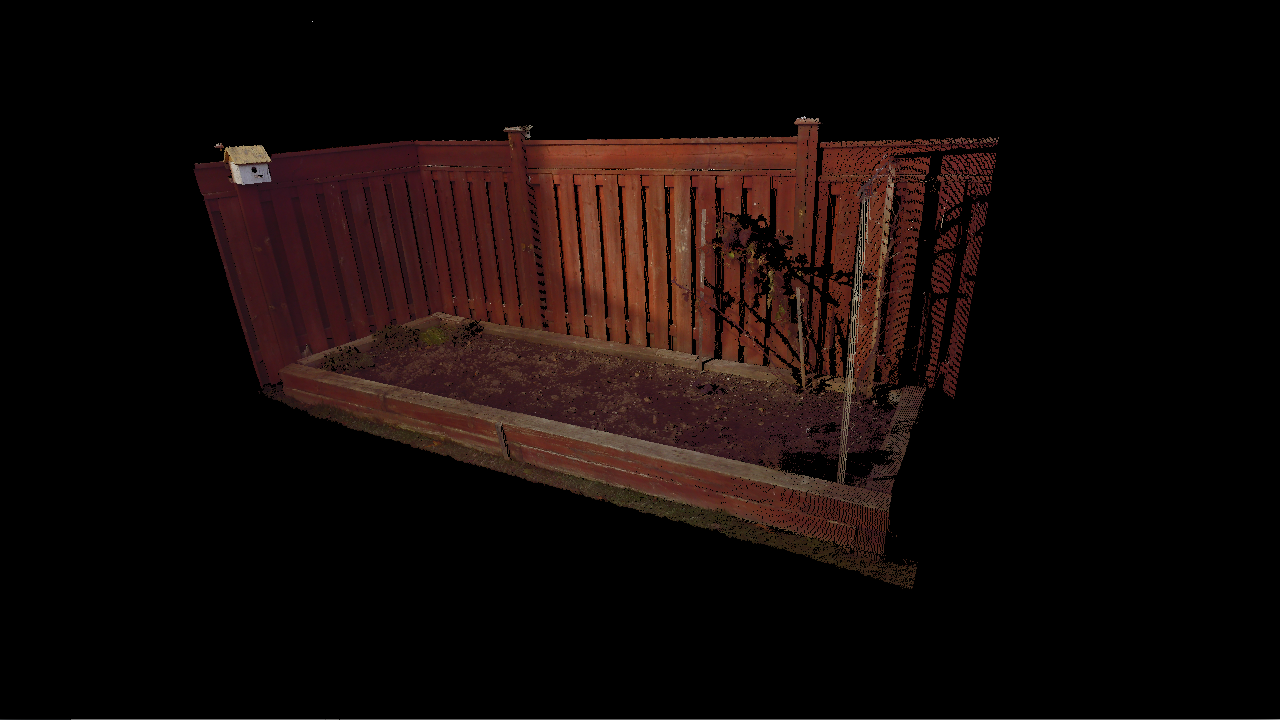
\includegraphics[keepaspectratio,width=\textwidth]{obrazky/mrak}
	\captionof{figure}{Pohled na načtené mračno}
	\label{mrak}
\end{figure}

\begin{figure}
	\centering
	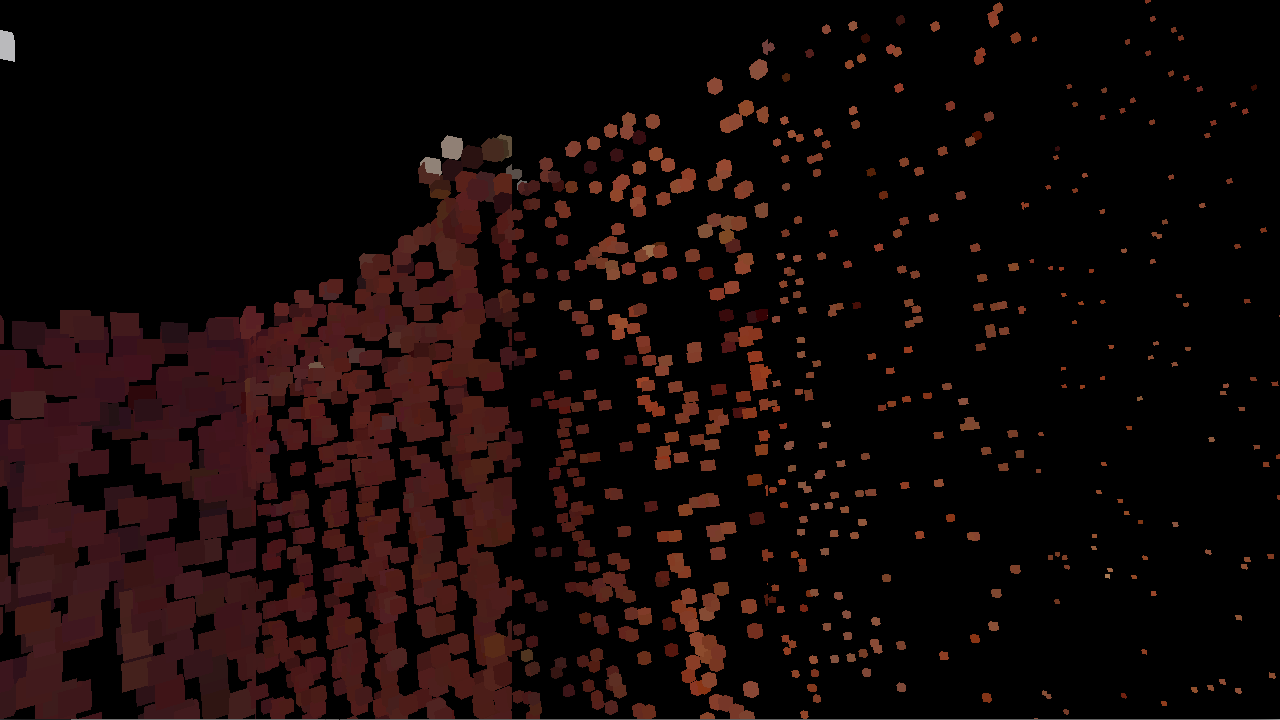
\includegraphics[keepaspectratio,width=\textwidth]{obrazky/velikosti}
	\captionof{figure}{Demonstrace změny velikosti bodů}
	\label{velikosti}
\end{figure}

\begin{figure}
	\centering
	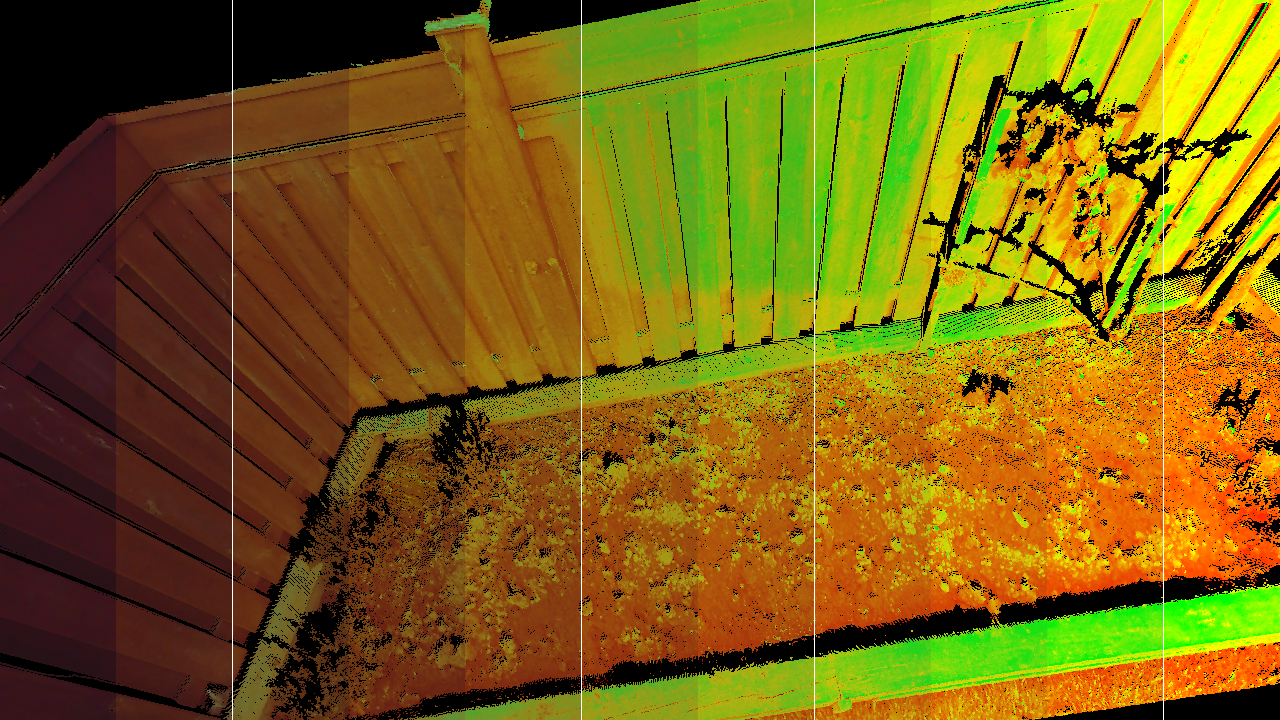
\includegraphics[keepaspectratio,width=\textwidth]{obrazky/skalar}
	\captionof{figure}{Demonstrace přimíchávání škály skalárního pole}
	\label{skalar}
\end{figure}

\FloatBarrier

\section{Ovládání programu}

Veškeré ovládání programu bylo nejprve implementováno pomocí klávesnice.

Pomocí kláves W a S se pohled posouvá po ose Z, A a D po ose X a Alt a mezerník po ose Y. Pomocí šipek nahrou a dolů se pohled natáčí podle osy X, pomocí šipek doleva a doprava podle Y a pomocí kláves Q a E se naklápí podle osy Z.

Klávesou R se velikost bodu zdvojnásobí, klávesou F sníží na polovinu. Klávesami T a G se plynule přechází mezi barvou mračna a skalárním polem.

Klávesou M se vyvolá menu. Šipkami nahoru a dolů se vybírají jednotlivé prvky v menu, výběr se potvrdí klávesou Enter, pro vrácení o úroveň nahoru klávesa Escape.

Program se uzavře stisknutím Escape mimo menu.

\begin{figure}
	\centering
	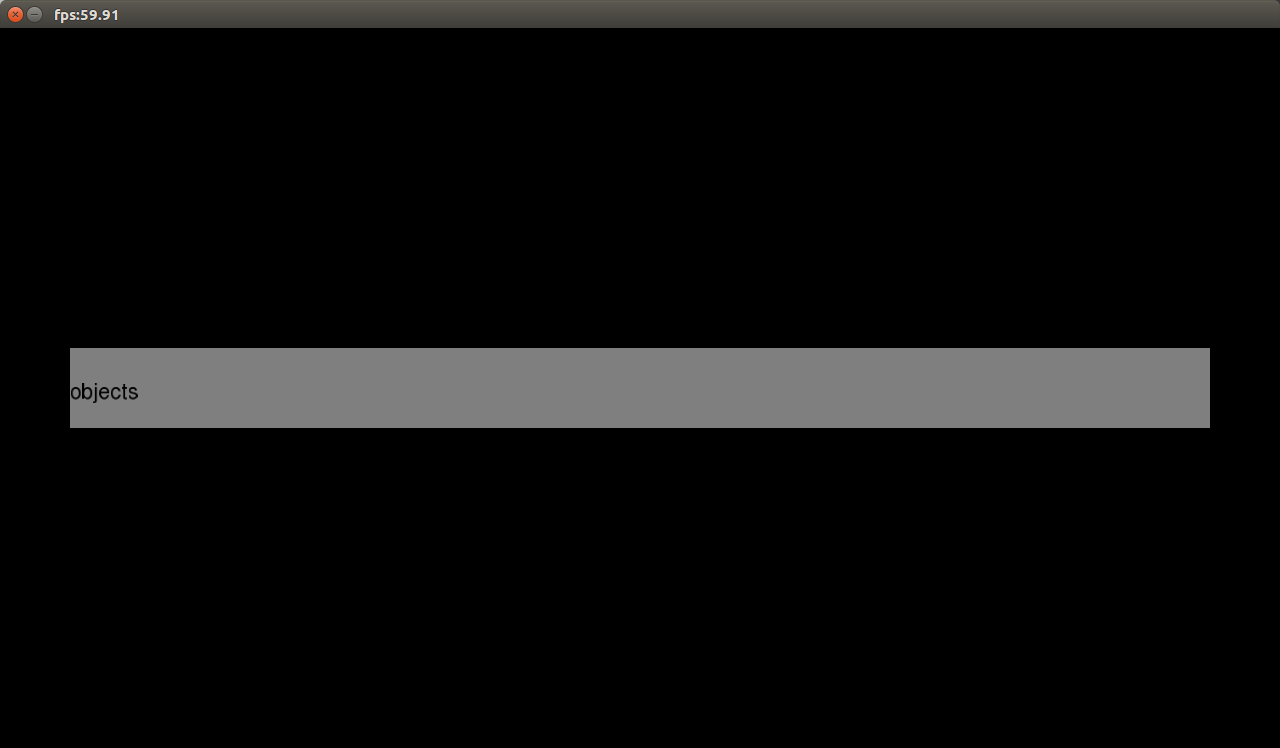
\includegraphics[keepaspectratio,width=\textwidth]{obrazky/objects}
	\captionof{figure}{Hlavní menu}
	\label{hlavni-menu}
\end{figure}

\begin{figure}
	\centering
	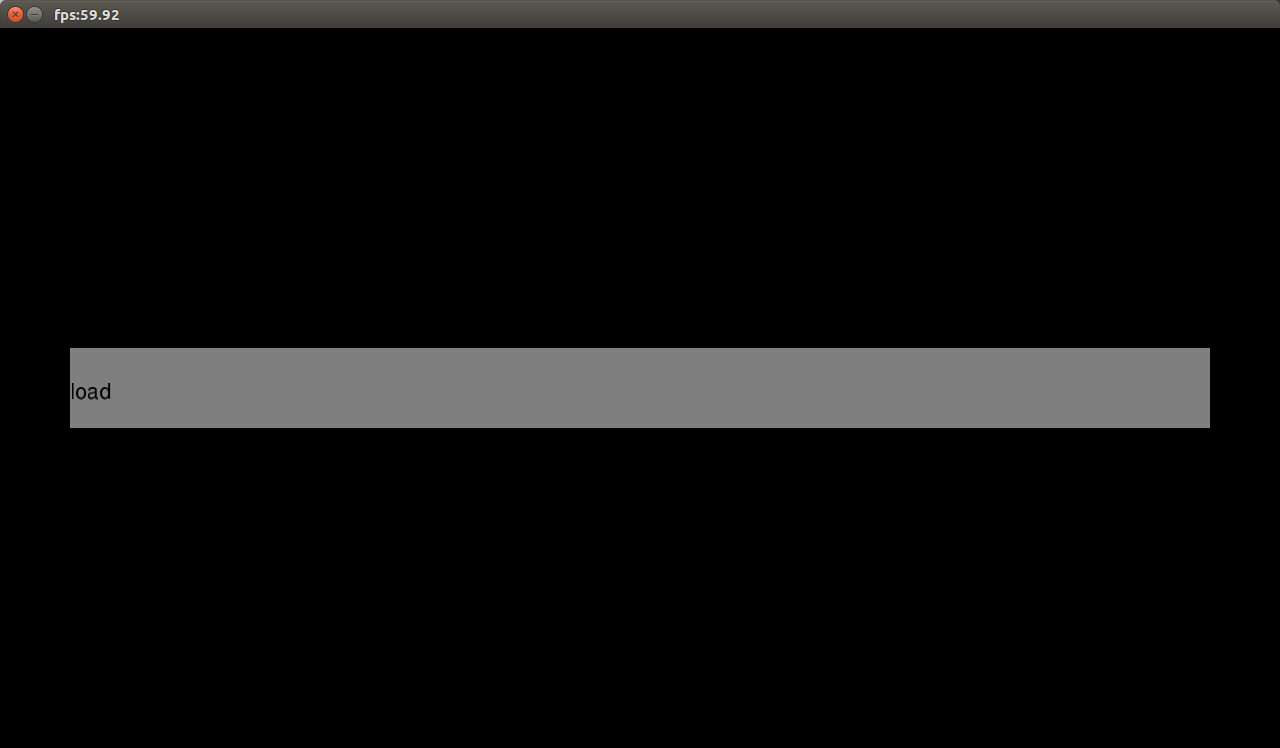
\includegraphics[keepaspectratio,width=\textwidth]{obrazky/prazdne-objekty}
	\captionof{figure}{Menu objekty}
	\label{objects}
\end{figure}

Po vyvolání menu lze vidět položku objects, viz obrázek \ref{hlavni-menu}, v ní je seznam všech načtených mračen do programu a položku load (obrázek \ref{objects}), pomocí ní lze načíst mračno. Pokud operátor vybere již načtené mračno, bude mít v nabídce možnost toto mračno odstranit.

Poté jsem implementoval částečné ovládání pomocí pravého ovladače.

Pro pohyb po scéně je nejprve nutné stisknout trigger, poté táhnout ovladačem a nakonec trigger uvolnit. Stisknutím horního tlačítka na pravém ovladači se vyvolá menu. Pohybem prstu po trackpadu se posouvá položkami v menu, triggerem se výběr potvrdí. Horním tlačítkem se také vrací na vyšší úroveň menu a menu uzavírá.


